\renewcommand{\thefootnote}{\fnsymbol{footnote}}

\chapter[Stochastic dominance and applications]%
 {Stochastic dominance and applications}%
\label{ch:L4}

% 3) Reset things so later footnotes go back to 1, 2, 3, …
%\setcounter{footnote}{0}
\renewcommand{\thefootnote}{\arabic{footnote}}

\section{Stochastic dominance}\label{sec:L4-intro}

We just developed an analysis of properties of expected utility preferences. However, we have not yet discussed relevant properties of lotteries, which is what we do now. As an example, one might want to have a language to say that a \textquote{lottery yields higher returns than another one}.

A simple way of capturing this idea is the following: for each given return, the probability of getting at least that return is higher in one lottery than in the other one. Formally, for each return \( x \), if \( F(x) \leq G(x) \), then the probability of getting at least \( x \) is higher in lottery \( F \) than in lottery \( G \), bacause the area \textquote{on the left} of \( F \) is smaller. In other words, the CDF of a \textquote{better} lottery lies everywhere below that of a “worse” one — meaning that, for any return \( x \), more probability mass lies above that return. This idea is captured by the concept of first-order stochastic dominance.

\begin{definition}\label{def:fosd}
	The lottery \( F \) \textbf{first-order stochastically dominates} \( G \) if

	\[
		F(x) \leq G(x) \quad \text{for all } x.
	\]
\end{definition}

As illustrated in Figure \ref{fig:fosd}, lottery \( F \) first-order stochastically dominates lottery \( G \) if its graph is always below the graph of lottery \( G \).

\begin{figure}[H]
	\centering
	\tikzset{every picture/.style={line width=0.75pt}} %set default line width to 0.75pt        

	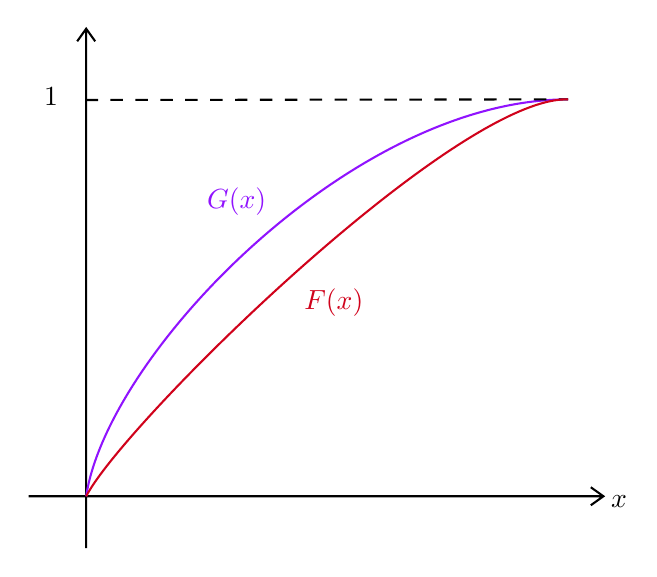
\begin{tikzpicture}[x=0.65pt,y=0.65pt,yscale=-1,xscale=1]
		%uncomment if require: \path (0,349); %set diagram left start at 0, and has height of 349

		%Shape: Axis 2D [id:dp8000510474681485] 
		\draw  (160,302.32) -- (479.48,302.32)(191.95,42.4) -- (191.95,331.2) (472.48,297.32) -- (479.48,302.32) -- (472.48,307.32) (186.95,49.4) -- (191.95,42.4) -- (196.95,49.4)  ;
		%Curve Lines [id:da5171104107126938] 
		\draw [color={rgb, 255:red, 144; green, 19; blue, 254 }  ,draw opacity=1 ]   (191.95,302.32) .. controls (203.57,223.81) and (339.39,81.68) .. (459.83,81.68) ;
		%Straight Lines [id:da9399220418666737] 
		\draw  [dash pattern={on 4.5pt off 4.5pt}]  (191.61,82.02) -- (459.83,81.68) ;
		%Curve Lines [id:da8164662036086425] 
		\draw [color={rgb, 255:red, 208; green, 2; blue, 27 }  ,draw opacity=1 ]   (191.95,302.32) .. controls (212.96,261.57) and (397.47,80) .. (459.83,81.68) ;

		% Text Node
		\draw (482.02,300.33) node [anchor=north west][inner sep=0.75pt]    {$x$};
		% Text Node
		\draw (166.81,73.24) node [anchor=north west][inner sep=0.75pt]    {$1$};
		% Text Node
		\draw (311.5,185.35) node [anchor=north west][inner sep=0.75pt]  [color={rgb, 255:red, 208; green, 2; blue, 27 }  ,opacity=1 ]  {$F( x)$};
		% Text Node
		\draw (257.47,128.87) node [anchor=north west][inner sep=0.75pt]  [color={rgb, 255:red, 144; green, 19; blue, 254 }  ,opacity=1 ]  {$G( x)$};


	\end{tikzpicture}
	\caption{Lottery \( F \) first-order stochastically dominates lottery \( G \).}
	\label{fig:fosd}
\end{figure}

There is a second way of capturing the idea: an individual with expected utility preferences should prefer lottery \( F \) to lottery \( G \) for any possibile utility function \( u \). Formally,

\begin{equation}\label{eq:fosd}
	\int u(x) dF(x) \geq \int u(x) d G(x) \quad \text{for every nondecreasing } u.
\end{equation}

The two criteria \eqref{def:fosd} and \eqref{eq:fosd} are equivalent, as stated by the following result.

\begin{proposition}\label{prop:fosd}
	Lottery \( F \) first-order stochastically dominates lottery \( G \) if and only if Equation \eqref{eq:fosd} holds.
\end{proposition}

Notice that first-order stochastic dominance is an \textit{incomplete} ordering over lotteries: there are pairs of lotteries \( (F, G) \) such that neither \( F \) first-order stochastically dominates \( G \) nor \( G \) first-order stochastically dominates \( F \).

First order stochastic dominance is a comparison of returns. We now develop a notion allowing us to compare riskiness. Again, we start from an intuitive idea: say that two lotteries have the same expected return, but a risk averter prefers one lottery to the other. Since the individual is risk averse, she must be preferring the less risky lottery. In this case, we say that the first lottery second-order stochastically dominates the second one.

\begin{definition}\label{def:sosd}
	The lottery \( F \) \textbf{second-order stochastically dominates} \( G \) with the same mean if

	\[
		\int u(x) d F(x) \geq \int u(x) dG(x) \quad \text{for every nondecreasing concave } u.
	\]
\end{definition}

Recall that if an expected utility maximiser has a concave utility function, he is risk averse, which explains the qualifier in Definition \ref{def:sosd}.

\section{Applications}

come va.

\paragraph{Things to read.} leggi \cite{mas-colellMicroeconomicTheory1995}.

\section{Exercises}

\begin{exercise}
	Prove one direction of Proposition \ref{prop:fosd}: show that if  Equation \eqref{eq:fosd} holds, then \( F \) first-order stochastically dominates \( G \) in the sense of Definition \ref{def:fosd}. (check \citet[p. 195]{mas-colellMicroeconomicTheory1995} if you are stuck)
\end{exercise}

\bibliographystyle{apacite}  % or another  style
\bibliography{references} % .bib file goes in ./bib/